\providecommand{\curso}{Octavo Básico A}
\providecommand{\colegio}{Colegio Divina Pastora}
\providecommand{\tituloDocumento}{Control 2}
\providecommand{\subtituloDocumento}{Diagramas de caja}

\documentclass{cdplf-prueba}

\begin{document}
%
\begin{tcbraster}[enhanced,raster columns=3,raster width=\linewidth,raster column skip=3pt,raster force size=false]
    \begin{caja}[title={\sffamily\scshape\bfseries Nombre},height=30pt,add to width=4cm]
    \end{caja}
    \begin{caja}[title={\sffamily\scshape\bfseries Puntaje},height=30pt,add to width=-2cm]
    \end{caja}
    \begin{caja}[title={\sffamily\scshape\bfseries Nota},height=30pt,add to width=-2cm]
    \end{caja}                    
\end{tcbraster}
%
\vspace*{10pt}

\begin{tcolorbox}[boxrule=1pt,colback=white,leftrule=3mm]
    \raggedright Determine el diagrama de caja que le corresponde a cada una de las
    tablas de frecuencia entregadas. No olvide colocar su respuesta en los lugares señalizados.        
\end{tcolorbox}

\subsection{}
    %% solución 3 9 13 16
    \vspace{10pt}
    \begin{center}
    \begin{tblr}{width=0.8\linewidth,colspec={X[1,c]X[3,c]X[3,c]X[3.5,c]},hlines,vlines,hline{2,Z} = {1}{-}{},hline{2,Z} = {2}{-}{},row{even}={black!10},
        row{1}={font=},rowsep=5pt,cells={valign=m}}
            &Frecuencia&Frecuencia Acumulada&Probabilidad Acumulada \\
        1   &   1  &    1   &   0.02 \\
        4   &   1  &    2   &   0.05 \\
        5   &   3  &    5   &   0.13 \\
        8   &   4  &    9   &   0.23 \\
        9   &   8  &    17   &   0.43 \\
        10  &   4  &    21  &   0.53 \\
        11  &   2  &    23  &   0.58 \\
        12  &   5  &    28  &   0.70 \\
        13  &   6  &    34  &   0.85    \\
        14  &   4  &    38  &   0.95 \\
        15  &   1  &    39  &   0.98 \\
        16  &   1  &    40  &   1    \\
    \end{tblr}
    \end{center}
    \vspace{30pt}
    \begin{center}
    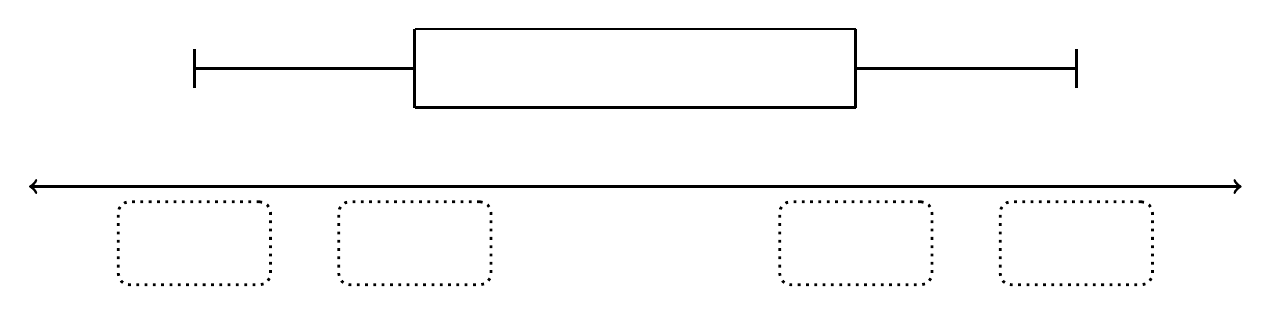
\begin{tikzpicture}[ampersand replacement=\&,line width=1pt,x=1.4cm]
        \draw[<->] (-5.5,0) -- (5.5,0);
        \draw[] (-4,1.25) -- (-4,1.75) (-2,1) -- (-2,2) (2,1) -- (2,2) (4,1.25) -- (4,1.75)%
            (-4,1.5) -- (-2,1.5) (2,1.5) -- (4,1.5) (-2,2) -- (2,2) (-2,1) -- (2,1);
        \node[draw,dotted,rounded corners,inner sep=15pt,text width=25pt,anchor=north,yshift=-5pt] at (-4,0) {};
        \node[draw,dotted,rounded corners,inner sep=15pt,text width=25pt,anchor=north,yshift=-5pt] at (-2,0) {};
        \node[draw,dotted,rounded corners,inner sep=15pt,text width=25pt,anchor=north,yshift=-5pt] at (2,0) {};
        \node[draw,dotted,rounded corners,inner sep=15pt,text width=25pt,anchor=north,yshift=-5pt] at (4,0) {};
    \end{tikzpicture}
    \end{center}

\subsection{}
    %% solución: {6, 8, 12, 18}
    \vspace{10pt}
    \begin{center}
    \begin{tblr}{width=0.8\linewidth,colspec={X[1,c]X[3,c]X[3,c]X[3.5,c]},hlines,vlines,hline{2,Z} = {1}{-}{},hline{2,Z} = {2}{-}{},row{even}={black!10},
        row{1}={font=},rowsep=5pt,cells={valign=m}}
                &   Frecuencia  &   Frecuencia Acumulada    &   Probabilidad Acumulada \\
                6  &       2       &                           &                          \\
                7  &       5       &                           &                          \\
                8  &       9       &                           &                          \\
                9  &       2       &                           &                          \\
                10  &      8       &                           &                          \\
                11  &      4       &                           &                          \\
                12  &      1       &                           &                          \\
                13  &      5       &                           &                          \\
                14  &      3       &                           &                          \\
                16  &      1       &                           &                          \\
                19  &      1       &                           &                          \\
            \end{tblr}
    \end{center}
    \vspace{30pt}
    \begin{center}
    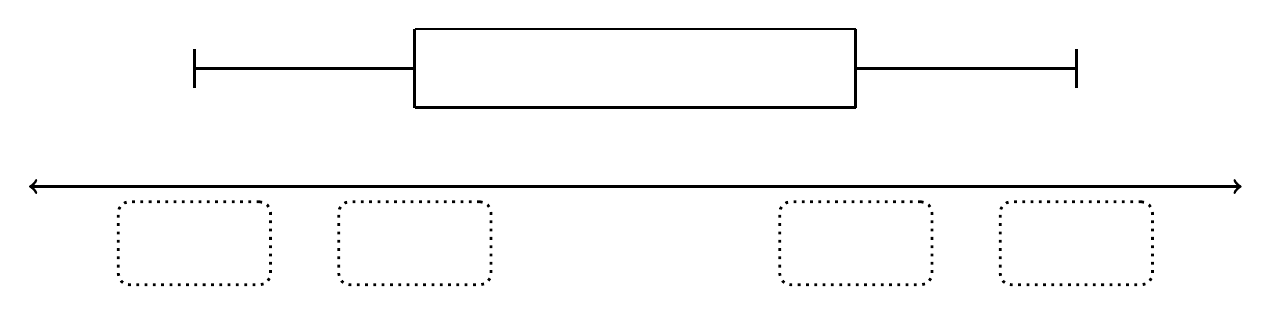
\begin{tikzpicture}[ampersand replacement=\&,line width=1pt,x=1.4cm]
        \draw[<->] (-5.5,0) -- (5.5,0);
        \draw[] (-4,1.25) -- (-4,1.75) (-2,1) -- (-2,2) (2,1) -- (2,2) (4,1.25) -- (4,1.75)%
            (-4,1.5) -- (-2,1.5) (2,1.5) -- (4,1.5) (-2,2) -- (2,2) (-2,1) -- (2,1);
        \node[draw,dotted,rounded corners,inner sep=15pt,text width=25pt,anchor=north,yshift=-5pt] at (-4,0) {};
        \node[draw,dotted,rounded corners,inner sep=15pt,text width=25pt,anchor=north,yshift=-5pt] at (-2,0) {};
        \node[draw,dotted,rounded corners,inner sep=15pt,text width=25pt,anchor=north,yshift=-5pt] at (2,0) {};
        \node[draw,dotted,rounded corners,inner sep=15pt,text width=25pt,anchor=north,yshift=-5pt] at (4,0) {};
    \end{tikzpicture}
    \end{center}

\end{document}